%\documentclass[a0paper,portrait]{baposter}
\documentclass[paperwidth=38in,paperheight=28in,landscape,fontscale=0.4]{baposter}

\usepackage{amssymb}
\setcounter{tocdepth}{3}
\usepackage{graphicx}

\usepackage{wrapfig}
\usepackage[normalem]{ulem}
\usepackage[USenglish]{babel} %francais, polish, spanish, ...
\usepackage[T1]{fontenc}
\usepackage[ansinew]{inputenc}
\usepackage{amsmath}
\usepackage{amsfonts}
%\usepackage[numbers]{natbib}
%\usepackage{relsize}
\usepackage{enumerate}

\usepackage[ruled]{algorithm2e}

\usepackage{url}  
\newcommand{\keywords}[1]{\par\addvspace\baselineskip
\noindent\keywordname\enspace\ignorespaces#1}


\newcommand{\adagrad}{{\sc AdaGrad}\ }

\newcommand{\xopt}{x_{\star}}
\newcommand{\Xopt}{X_{\star}}
\newcommand{\sspace}{\mathcal{S}}
\newcommand{\fracpartial}[2]{\frac{\partial #1}{\partial  #2}}
\newcommand{\bmat}{\begin{pmatrix}}
\newcommand{\emat}{\end{pmatrix}}
\newcommand{\N}{\mathbb{N}}
\newcommand{\Z}{\mathbb{Z}}
\newcommand{\R}{\mathbb{R}}
\newcommand{\Order}{\mathcal{O}}
\newcommand{\erf}{\operatorname{erf}}
\newcommand{\diag}{\operatorname{diag}}
\newcommand{\Symm}{\mathcal{S}}
\newcommand{\PD}{\mathcal{P}}
\newcommand{\Normal}{\mathcal{N}}
\newcommand{\Expectation}{\mathbb{E}}
\newcommand{\Var}{\mathbb{V}\operatorname{ar}}
\newcommand{\trace}{\operatorname{tr}}
\newcommand{\corresponds}{\mathop{\widehat=}}
\newcommand{\invA}{B}
\newcommand{\logDetA}{\ell}
\newcommand{\logDensity}{\rho}
\newcommand{\Mean}{\boldsymbol{\mu}}
\newcommand{\Cov}{\mathbf{\Sigma}}
\newcommand{\Tail}{\boldsymbol{\tau}}
\newcommand{\sqCov}{\mathbf{A}}
\newcommand{\sqCovB}{\mathbf{B}}
\newcommand{\nsqCov}{\mathbf{M}}
\newcommand{\nCenter}{\boldsymbol{\delta}}
\newcommand{\covs}{\boldsymbol{\sigma}}
\newcommand{\Sample}{\mathbf{z}}
\newcommand{\SampleTwo}{\mathbf{z'}}
\newcommand{\nSample}{\mathbf{s}}
\newcommand{\transp}{^{\top}}
\newcommand{\popsize}{\lambda}
\newcommand{\prevTheta}{\theta^{\prime}}
\newcommand{\fisher}{\mathbf{F}}
\newcommand{\natG}{\widetilde{\nabla}_{\theta} J}
\newcommand{\idM}{\mathbb{I}}

\newcommand{\params}{\boldsymbol{\theta}}
\newcommand{\grad}{\nabla_{\params}}
\newcommand{\gradw}{\widehat{\nabla_{\params}}}
\newcommand{\gradj}{\nabla_{\theta_{j}}}
\newcommand{\gradz}{\nabla_{\theta_{0}}}
\newcommand{\gradjj}[1]{\nabla_{\params_{#1}}}
\newcommand{\hess}{\mathbf{H}}
\newcommand{\cent}{\mathbf{c}}


\newcommand{\hatg}{\overline{g_i}}
\newcommand{\hatv}{\overline{v_i}}
\newcommand{\hath}{\overline{h_i}}
\newcommand{\hatvg}{\overline{l}}

\usepackage{color}
\definecolor{dkgreen}{rgb}{0.1,0.4,0}
\definecolor{orange}{rgb}{0.8,0.4,0}
\definecolor{nyupurple}{rgb}{0.5,0.0,0.9}
\definecolor{nyupurplelight}{rgb}{0.9,0.8,1}
\definecolor{violet}{rgb}{1,0.,0.5}
\newcommand{\comm}[1]{\textcolor{violet}{#1}} % comment about the text
\newcommand{\eemph}[1]{\textcolor{violet}{#1}} % comment about the text
\newcommand{\later}[1]{\textcolor{nyupurple}{#1}}  % complete later, flash out, extensions

\makeatletter

\def\Ddots{\mathinner{\mkern1mu\raise\p@
\vbox{\kern7\p@\hbox{.}}\mkern2mu
\raise4\p@\hbox{.}\mkern2mu\raise7\p@\hbox{.}\mkern1mu}}
\makeatother

\newcommand{\compresslist}{%
\setlength{\itemsep}{1pt}%
\setlength{\parskip}{0pt}%
\setlength{\parsep}{0pt}%
}


\begin{document}
\begin{poster}%
  % Poster Options
  {
  % Show grid to help with alignment
  grid=false,
  % Column spacing
  columns=4,
  colspacing=1.3em,
  % Color style
  bgColorOne=white,
  bgColorTwo=white,
  borderColor=nyupurplelight,
  headerColorOne=nyupurplelight,
  headerColorTwo=nyupurplelight,
  headerFontColor=nyupurple,
  boxColorOne=white,
  boxColorTwo=white,
  % Format of textbox
 textborder=roundedleft,
  % Format of text header
  eyecatcher=true,
  headerborder=closed,
  headerheight=0.17\textheight,
%  textfont=\sc, An example of changing the text font
  headershape=roundedright,
  %headershade=shadelr,
  headerfont=\Large\bf\textsc, %Sans Serif
  textfont={\setlength{\parindent}{0em}},
  %boxshade=plain,
%  background=shade-tb,
  background=plain,
  linewidth=2pt
  }
  % Eye Catcher
  { 
\includegraphics[height=10.0em]{torch2.jpg}
   } 
  % Title
  {\vspace{0.2em}\bf\textsc{
  Saturating Auto-Encoders
  }
%  \\ {\Large   Adaptive Learning Rates for Stochastic Gradients  }
  \vspace{0.4em}
  }
  % Authors
  {{\bf\textsc{Rostislav Goroshin and Yann LeCun}}
  \\ %\vspace{0.3em}
  Courant Institute of Mathematical Sciences, 
  New York University
  %715 Broadway, 10003, New York
  \\
  \url{{goroshin,yann}@cims.nyu.edu}
}
  % University logo
  {% The makebox allows the title to flow into the logo, this is a hack because of the L shaped logo.
    
\includegraphics[height=10.0em]{torch2.jpg}
  }
  
\headerbox{\large Auto-Encoders Learn Manifolds}{name=manifold,column=0,row=0}{
\begin{itemize} \compresslist
\item Data lies on a low-dimensional manifold embedded in a higher dimensional ambient space 
\item Reconstruction objective ensures low reconstruction error in portions of the input space where data is densely distributed
\item {\bf Regularizers should raise reconstruction error for inputs not near the data manifold} 
\item Analogous to minimizing the partition function in max-likelihood models
\begin{center}     
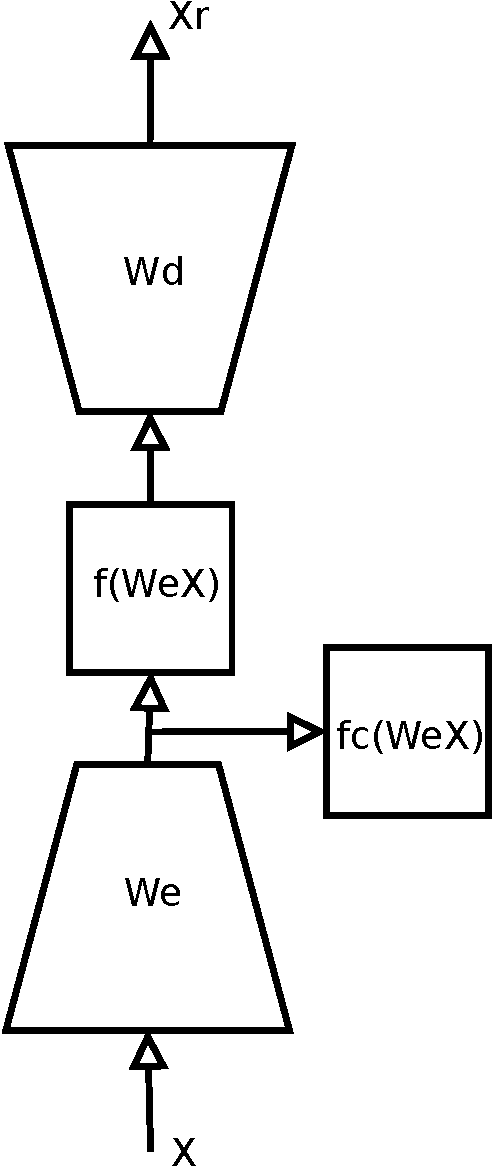
\includegraphics[height=20.0em]{SATAE.pdf}
\end{center} 
\end{itemize} 
}


\headerbox{Latent State Regularization}{name=lsreg,column=0,below=manifold}{
 	Latent state regularization is a method of introducing an information bottleneck, which is more intuitive than regularizing the weights directly.  

    \begin{itemize}\compresslist
      \item Unsupervised Setting: Sparsity ($L_1$) and Contractive Regularization
      \item Supervised Setting: Penalize the Surface Area of the Decision Boundary  
    \end{itemize}
}

\headerbox{Toy-Manifold Example}{name=toy,column=0,below=lsreg}
{
\begin{center}     
Unregularized \hspace{15mm} Regularized \\
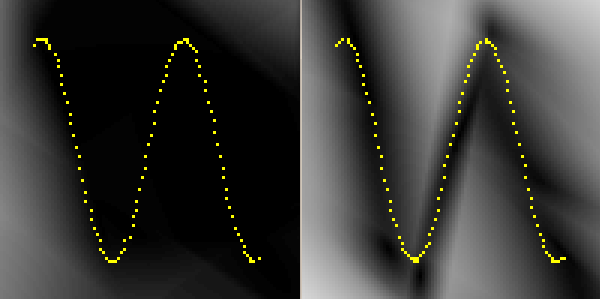
\includegraphics[scale=0.4]{toy_shrink.png}\\
%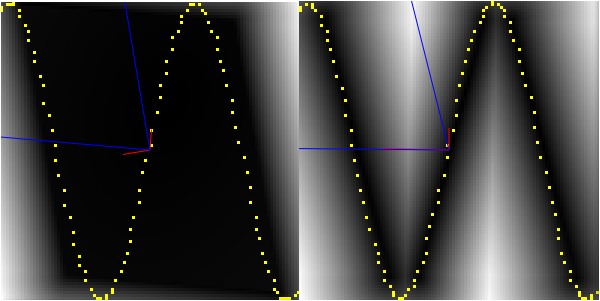
\includegraphics[scale=0.2]{sat_linear_toy.png}
\end{center} 
}
 

\headerbox{Regularization via Saturation}{name=comp,column=1,row=0}
{
\begin{itemize}\compresslist
\item Consider activation functions with flat (zero-gradient) regions 
\item These activation functions lose their ability to reconstruct the input when activations occur in the flat regions
\item Reconstruction error will increase quadratically as we move away from the manifold 
\item We associate with each activation function a complimentary function which encourages activations in the flat regions 
\end{itemize} 
\begin{center}     
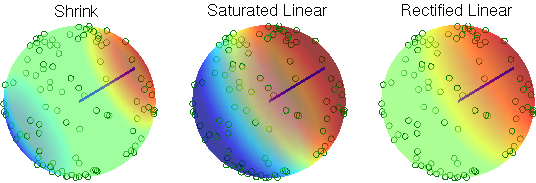
\includegraphics[scale=0.43]{viz_nonlin.png} \\
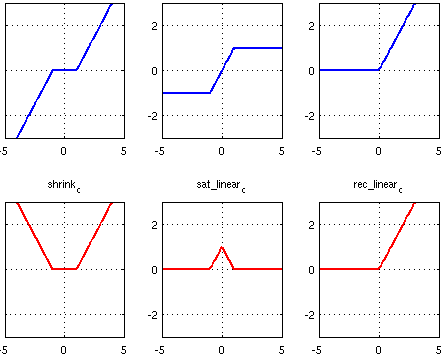
\includegraphics[scale=0.53]{compliments.png} \vspace*{2mm} 
\emph{\uline {Complimentary Function}} \\
$f_c(z) = \inf_ {z' \in S} |z-z'|$ \\
\vspace{2mm} 
\emph{\uline {Loss Functional}} 
%\setlength{\jot}{1mm} 
\begin{multline} \nonumber 
%\begin{split}
L =\sum_{x \in D} \frac{1}{2} \|x-\left(W^d f(W^e x+B^e)+B^d\right)\|^2 \\ 
 + ~\alpha \sum_{i=1}^{d_h}f_c(W^e_i x + b^e_i)
%\end{split}
\end{multline} 
%\emph{\uline {$L_1$-Equivalence}} \\
\end{center}  
}

\headerbox{References}{name=ref,column=1,below=comp, span=2}
{
\footnotesize{
1. Rifai, S. and Vincent, P. and Muller, X. and Glorot, X. and Bengio, Y. Contractive auto-encoders: Explicit invariance during feature extraction, {\em Proceedings of the Twenty-eight International Conference on Machine Learning,  ICML 2011}\\
2. Karol Gregor and Yann LeCun: Learning Fast Approximations of Sparse Coding, Proc. {\em International Conference on Machine learning (ICML'10)}, 2010\\
3. Marc'Aurelio Ranzato, Christopher Poultney, Sumit Chopra and Yann LeCun. Efficient Learning of Sparse Representations with an Energy-Based Model, in J. Platt et al. (Eds), {\em(NIPS 2006)}, 19, MIT Press, 2006.}

}

\headerbox{SATAE-shrink on CIFAR-10}{name=shrink,column=2,row=0, span=1}
{
\begin{center} 
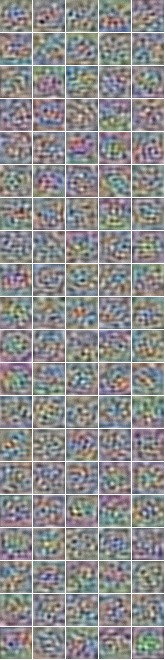
\includegraphics[scale=0.366]{shrink_unreg.png}
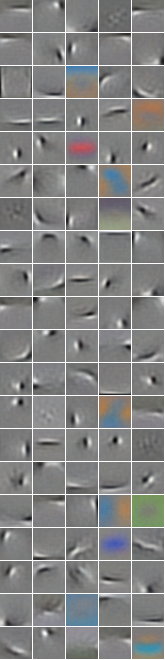
\includegraphics[scale=0.366]{CIFAR_shrink01.png}	
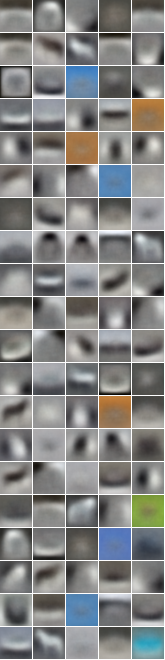
\includegraphics[scale=0.366]{CIFAR_shrink05.png}	
\end{center} 
}

\headerbox{SATAE-sat-linear on CIFAR-10}{name=satlinear,column=2,below=shrink, span=1}
{
\begin{center} 
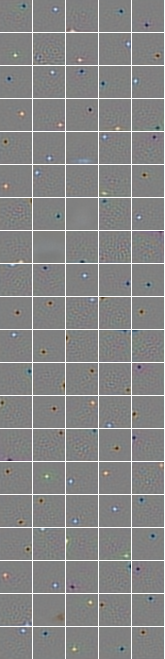
\includegraphics[scale=0.366]{sat_linear0.png}
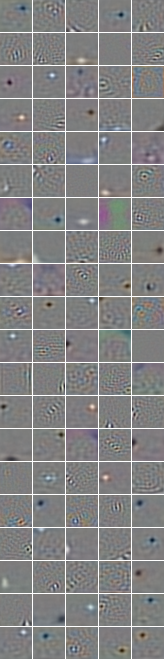
\includegraphics[scale=0.366]{sat_linear1.png}	
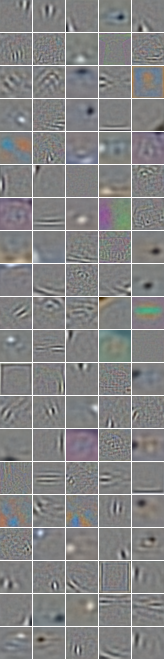
\includegraphics[scale=0.366]{sat_linear2.png}	
\end{center} 
}

\headerbox{Progressively Increasing $\alpha$}{name=proreg,column=3,row=0, span=1}
{
\begin{center}
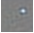
\includegraphics[scale=1]{1.png} 
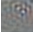
\includegraphics[scale=1]{2.png}

\includegraphics[scale=1]{3.png}
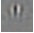
\includegraphics[scale=1]{4.png}
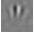
\includegraphics[scale=1]{5.png}\\
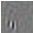
\includegraphics[scale=1.02]{horse/1.png} 
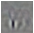
\includegraphics[scale=1.02]{horse/2.png}

\includegraphics[scale=1.02]{horse/3.png}
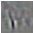
\includegraphics[scale=1.02]{horse/4.png}
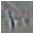
\includegraphics[scale=1.02]{horse/5.png}\\

\includegraphics[scale=2]{horse0.png}
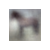
\includegraphics[scale=2]{horse1.png} 
\end{center}

}

\headerbox{\large Relation to Other Regularizers}{name=disc,column=3,below=proreg, span=1}
{

\emph{\uline {Connection to Sparse-Auto-Encoders}} \vspace{2mm} \\ 
Note that $shrink_c(W^e x + b^e) =  abs(shrink(W^e x + b^e))$. For $shrink$-nonlinearity, our regularizer corresponds to $L_1$ penalty on the activations.\\ \\
\emph{\uline {Connection to Contractive-Auto-Encoders}} \\
\begin{equation}
\nonumber
\sum_{ij} \left(\frac{\partial h_i}{\partial x_j} \right)^2 = \sum_i ^{d_h} \left(f'(\sum_{j=1}^d W^e_{ij}x_j + b_i)^2 \| W^e_i \| ^2 \right)
\end{equation}  
The first term in the above equation tries to adjust the weights so as to push the activations into the low gradient (saturation)
regime of the nonlinearity, but is only defined for differentiable activation functions. Therefore the
CAE indirectly encourages operation in the saturation regime. \\ \\
}

\headerbox{Extension to $C^1$}{name=ext,column=3,below=disc, span=1}
{
We employ the concept of average variation over a finite interval to extend the definition of complimentary activation functions to differentiable functions.
\begin{center} 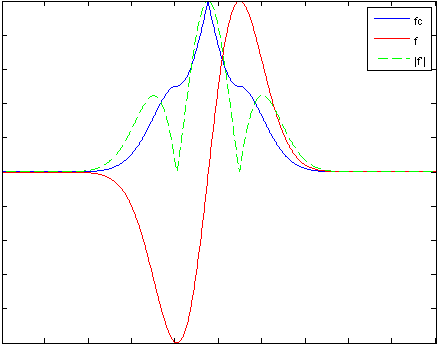
\includegraphics[scale=0.4]{diff_cc.png} \end{center} 
}


\end{poster}
\end{document}
